\documentclass[10pt]{article}

\usepackage[letterpaper,margin=0.82in]{geometry}
\usepackage{amsmath,amssymb}
\usepackage{booktabs}
\usepackage{graphicx}
\usepackage{microtype}
\usepackage{xcolor}
\usepackage{hyperref}
\usepackage{url}
\usepackage{enumitem}
\usepackage{placeins}
\usepackage{float}
\usepackage[font=small,labelfont=bf]{caption}

\graphicspath{{papers/figures/}{figures/}}
\hypersetup{
  colorlinks=true,
  linkcolor=blue!50!black,
  urlcolor=blue!60!black,
  citecolor=blue!50!black,
  pdftitle={Reconstruction Without Pairwise Distances},
  pdfauthor={Igor Rivin}
}
\setlength{\parindent}{0pt}
\setlength{\parskip}{0.48em}
\setlist{nosep,leftmargin=1.5em}
\newcommand{\AEmethod}{\textsc{AE}}
\newcommand{\R}{\mathbb{R}}
\newcommand{\ind}{\mathbf{1}}

\title{\textbf{Reconstruction Without Pairwise Distances:}\\
       A Large-Scale Comparison of Autoencoders, DiRe, and UMAP}
\author{Igor Rivin}
\date{13 July 2026}

\begin{document}
\maketitle

\begin{abstract}
Graph-based dimension-reduction methods explicitly construct and optimize
relationships between observations.  A reconstruction autoencoder instead learns from
individual input vectors using only mean-squared error.  We compare these approaches at
target widths $d\in\{2,8\}$ on 723,457 arXiv paper embeddings and one million Wikipedia
paragraph embeddings.  All reducers receive the same row-normalized data and are
evaluated over three seeds using sample-conditional neighborhood fidelity, sampled
global-distance fidelity, local decodability, label- or group-aware diagnostics, sampled
persistence-derived diagnostics, and synchronized fit time.

No method dominates the completed cells.  At arXiv width two, the autoencoder leads the
rank-aware local scores, UMAP gives the best category prediction, and DiRe gives the
lowest sampled Betti-curve discrepancies.  At width eight, the autoencoder leads every
reported geometric score while UMAP still gives the best category prediction.  On the
Wikipedia corpus, width two divides the geometric columns among all three methods, while
at width eight the autoencoder leads the local, distance-order, and decoding scores but
not stress; DiRe gives the lowest global-distance stress at both widths and UMAP most
strongly groups paragraphs from the same article.  A separate controlled check on
manifolds of known dimension
finds that rounded TwoNN and autoencoder-elbow estimates agree exactly in four of nine
seeded trials and are within one dimension in all nine, with interpretable differences
between local and global reconstructive dimension.

The sampled topology comparison is similarly conditional on corpus and width.  DiRe
leads both Betti-curve discrepancies for arXiv at width two; at width eight the
autoencoder leads $\beta_0$ and DiRe leads $\beta_1$.  On Wikipedia, DiRe leads
$\beta_0$ and the autoencoder leads $\beta_1$ at width two, while the autoencoder leads
both at width eight.  A paired BF16-autocast sensitivity check preserves reconstruction
and shared-metric quality under prespecified practical margins.  It nearly halves
Wikipedia training time, but slightly slows the smaller arXiv network, showing that
mixed-precision speedup depends on whether dense computation amortizes its overhead.
\end{abstract}

\section{Why compare pointwise reconstruction with graph methods?}

For a fixed architecture and epoch budget, an autoencoder's work is linear in the number
of observations \cite{hinton2006}:
\[
  O\!\left(E N\sum_{\ell}w_{\ell}w_{\ell+1}\right),
\]
where $E$ is the number of epochs and $w_\ell$ are layer widths.  It never constructs a
pairwise distance matrix or a neighborhood graph.  DiRe and UMAP
\cite{dire,umap}, by contrast, begin from neighbor relationships.  Exact neighbor
construction would have quadratic scaling, so
their scalable implementations use approximate-nearest-neighbor indices and then optimize
a sparse graph.  That avoids $N^2$ storage and work, but introduces indexing, sampling,
and irregular memory access.  Dense autoencoder matrix multiplications are particularly
favorable on a large GPU.

This computational distinction does not imply that reconstruction preserves the geometry
needed by a particular application.  The central empirical question is therefore not
whether one method has a universally better score, but which structure each objective
retains.

\section{Data, reducers, and protocol}

\begin{table}[ht]
\centering
\small
\begin{tabular}{lrrrll}
\toprule
Corpus & Rows & Input $D$ & Target $d$ & Label field & Label interpretation\\
\midrule
arXiv & 723,457 & 384 & $2,8$ & primary category & subject category\\
Wikipedia & 1,000,000 & 1,024 & $2,8$ & article URL & same-article group\\
\bottomrule
\end{tabular}
\caption{The two large embedding corpora.  Wikipedia URLs are group identifiers, not a
topic taxonomy analogous to arXiv categories.}
\label{tab:data}
\end{table}

The arXiv matrix contains mean-pooled \texttt{BAAI/bge-small-en-v1.5} paper
embeddings \cite{bge}.  The Wikipedia matrix is the first million rows of the English
configuration of \texttt{CohereLabs/wikipedia-2023-11-embed-multilingual-v3}
\cite{coherewiki}.

Every input row is converted to float32 and normalized to unit Euclidean norm.  Each
method receives the complete normalized matrix at both $d=2$ and $d=8$, with
reducer/training seeds 0, 1, and 2.  Evaluation samples and sampled pairs are held fixed
across methods, target widths, and seeds.  DiRe and UMAP fitting, and all
neighborhood-based evaluations, use $k=16$; autoencoder fitting has no neighborhood
parameter.  The comparisons are transductive: every reported layout is fitted on the
full corpus being evaluated.

\paragraph{Autoencoder.}
For encoder $f_\theta$ and decoder $g_\phi$, training minimizes only elementwise
reconstruction MSE,
\begin{equation}
  \mathcal{L}(\theta,\phi)
  =\frac{1}{ND}\sum_{i=1}^{N}
    \left\|x_i-g_\phi\!\left(f_\theta(x_i)\right)\right\|_2^2.
  \label{eq:ae-loss}
\end{equation}
There is no label, pairwise-distance, neighborhood, contrastive, or topology term.
Hidden layers use SiLU activations; bottleneck and output layers are linear.  The
architectures are
\[
384\!\to\!256\!\to\!128\!\to\!32\!\to\!d\!\to\!32\!\to\!128\!\to\!256\!\to\!384
\]
for arXiv and
\[
1024\!\to\!512\!\to\!256\!\to\!64\!\to\!d\!\to\!64\!\to\!256\!\to\!512\!\to\!1024
\]
for Wikipedia.  As $d$ changes from two to eight, their parameter counts range from
271,682 to 272,072 and from 1,346,434 to 1,347,208, respectively.
AdamW uses learning rate $10^{-3}$ and weight decay $10^{-5}$, with batches of 32,768
rows.  The primary comparison uses float32 arithmetic; a separate BF16 sensitivity arm
is reported below.

Five percent of the rows select an epoch count under a 200-epoch cap and patience 15.
A freshly initialized model is then refit on all rows for the selected number of epochs.
The autoencoder is neither pretrained nor recycled between corpora, target widths, or
seeds.

\paragraph{DiRe and UMAP.}
DiRe 0.3.1 uses its cuVS implementation, with PCA initialization, 128 layout
iterations, and an automatically selected approximate-neighbor index.  cuML UMAP 26.06
uses Euclidean distance, spectral initialization, \texttt{min\_dist}$=0.1$, and
\texttt{spread}$=1$.  Native UMAP inverse transformation is disabled because its CPU
Delaunay stage is not a scale-safe operation for these corpora.

\paragraph{Hardware and timing.}
Reducer runs use a single NVIDIA GH200, RAPIDS/cuML 26.06, PyTorch 2.11, and three
independent reducer/training seeds.  Persistence calculations use Ripser 0.6.14 and
FastDTW 0.3.4 in the RAPIDS 26.04 environment because those packages were unavailable in
the 26.06 environment.  CUDA synchronization brackets every reported fit.  DiRe and UMAP
time their synchronized \texttt{fit\_transform}; autoencoder time includes GPU staging,
validation-based training, fresh full-data refitting, full-corpus encoding, and native
reconstruction statistics.  Source loading, row normalization, library import, downstream
comparison metrics, and the final layout-file flush are outside ``fit.''  One-time data
preparation took 2.58 seconds for arXiv and 10.05--14.59 seconds across the two Wikipedia
runs; it may be reused across target widths.

\section{Evaluation metrics}

Let $X=\{x_i\}\subset\R^D$ be the normalized input and
$Y=\{y_i\}\subset\R^d$ a layout.  Neighborhood metrics use Euclidean distance and
$k=16$.  Their $O(n_s^2)$ rank calculations are performed within a declared fixed sample,
not the complete corpus: a label-stratified 5,000-paper sample for arXiv and a uniform
3,000-paragraph sample for Wikipedia.  Wikipedia has 153,264 URL groups, more than the
number of sample slots, so label stratification is not possible.  Identical sample indices
are used for all methods, target widths, and reducer seeds.

\subsection{Neighborhood fidelity}

For a sampled point $i$, let $N_X^k(i)$ and $N_Y^k(i)$ be its $k$ nearest neighbors in
input and layout space, and let $r_X(i,j)$ and $r_Y(i,j)$ be the corresponding full
within-sample ranks.  Define the introduced and lost neighbor sets
\[
 U_k(i)=N_Y^k(i)\setminus N_X^k(i),\qquad
 V_k(i)=N_X^k(i)\setminus N_Y^k(i).
\]
Trustworthiness \cite{trust} penalizes false neighbors introduced by the layout:
\begin{equation}
T(k)=1-\frac{2}{n_s k(2n_s-3k-1)}
 \sum_{i=1}^{n_s}\sum_{j\in U_k(i)}\bigl(r_X(i,j)-k\bigr).
\label{eq:trust}
\end{equation}
Continuity is reversed trustworthiness and penalizes input neighbors lost by the layout:
\begin{equation}
C(k)=1-\frac{2}{n_s k(2n_s-3k-1)}
 \sum_{i=1}^{n_s}\sum_{j\in V_k(i)}\bigl(r_Y(i,j)-k\bigr).
\label{eq:continuity}
\end{equation}
Both approach one for strong local fidelity.  Exact neighbor overlap is
\begin{equation}
O(k)=\frac{1}{n_s k}\sum_{i=1}^{n_s}
 \left|N_X^k(i)\cap N_Y^k(i)\right|.
\label{eq:overlap}
\end{equation}
Unlike trustworthiness and continuity, overlap gives no partial credit when a missed or
introduced neighbor has nearly the correct rank.

\subsection{Sampled global distances}

For 200,000 fixed, independently sampled non-self pairs $P$, with pair repetitions
allowed, write
\[
 \delta_{ij}=\|x_i-x_j\|_2,\qquad d_{ij}=\|y_i-y_j\|_2.
\]
Pair Spearman correlation $\rho_S$ is the ordinary correlation of the midranks of
$\{\delta_{ij}\}$ and $\{d_{ij}\}$.  The scale-aligned normalized stress is
\begin{equation}
 S=\left[
 \frac{\sum_{(i,j)\in P}(\delta_{ij}-a d_{ij})^2}
      {\sum_{(i,j)\in P}\delta_{ij}^2}
 \right]^{1/2},\qquad
 a=\frac{\sum_{(i,j)\in P}\delta_{ij}d_{ij}}
          {\sum_{(i,j)\in P}d_{ij}^2}.
\label{eq:stress}
\end{equation}
Higher $\rho_S$ and lower $S$ are preferable.  Equation~\eqref{eq:stress} is a
through-origin least-squares scale alignment; it is not Kruskal Stress-1 or a full
Procrustes fit.

\subsection{Shared local-decoding probe}

A separate sample---10,000 rows for arXiv and 5,000 for Wikipedia---is split 80/20.  The
training layout is whitened, retaining covariance eigenvectors with
$\lambda_j>\max(10^{-8}\lambda_{\max},\epsilon)$.  A distance-weighted 16-neighbor
regressor predicts all coordinates of $x$ from the whitened layout.  With training and
test folds $A$ and $B$,
\begin{equation}
 \operatorname{DecodeNMSE}
 =\frac{\sum_{i\in B}\|x_i-\widehat{x}(y_i)\|_2^2}
        {\sum_{i\in B}\|x_i-\bar{x}_A\|_2^2}.
\label{eq:decode}
\end{equation}
This shared transductive probe compares all reducers.  It is neither the autoencoder's
native decoder error nor an out-of-corpus generalization test.

\subsection{Labels and article groups}

For arXiv, categories occurring at least five times in the fixed metric sample are kept,
leaving 4,857 rows and 71 categories.  A fixed stratified 80/20 split trains a
distance-weighted 16-neighbor classifier in layout space.  We report ordinary accuracy
and balanced accuracy, the mean per-category recall.  Labels are never supplied to a
reducer.

For Wikipedia, a URL identifies paragraphs from the same article.  The 3,000 fixed
anchors query the complete one-million-row layout.  Let $G_i$ be the rows sharing anchor
$i$'s URL, and let $m_i=|N_Y^{16}(i)\cap G_i|$.  Empty and full-corpus-singleton groups are
excluded, leaving an eligible set $E$ of 2,895 anchors.  We report
\begin{align}
 \operatorname{Purity@16}&=\frac1{|E|}\sum_{i\in E}\frac{m_i}{16},\\
 \operatorname{Hit@16}&=\frac1{|E|}\sum_{i\in E}\ind[m_i>0],\\
 \operatorname{TrRecall@16}&=\frac1{|E|}\sum_{i\in E}
       \frac{m_i}{\min(16,|G_i|-1)}.
 \label{eq:groups}
\end{align}
The last quantity is explicitly a \emph{truncated} recall: it can reach one for a large
article after retrieving 16 mates, even if additional same-article paragraphs remain.

\subsection{Native autoencoder reconstruction}

For the final refitted model, native reconstruction is summarized by
\[
 \operatorname{NMSE}_{\AEmethod}
 =\frac{\sum_i\|x_i-g_\phi(f_\theta(x_i))\|_2^2}
        {\sum_i\|x_i-\bar{x}\|_2^2}.
\]
Writing $\hat x_i=g_\phi(f_\theta(x_i))$, mean reconstruction cosine is
\[
 \operatorname{ReconCos}_{\AEmethod}
 =\frac1N\sum_{i=1}^N
   \frac{\hat x_i^\top x_i}{\max(\|\hat x_i\|_2,10^{-12})}.
\]
The usual factor $\|x_i\|_2$ is one because all benchmark rows are nonzero and normalized.
These are autoencoder-only diagnostics; Equation~\eqref{eq:decode} is the cross-method
comparison.

\subsection{Controlled intrinsic-dimension cross-check}

The fixed-width benchmark asks how well a chosen $d$ preserves structure; it does not
itself estimate an intrinsic dimension.  We therefore run a separate controlled check
on three 600-point manifolds whose local dimensions are known: a rank-three Gaussian
linear subspace, a circle, and a noise-free Swiss roll.  Each is orthogonally embedded
in $\R^{10}$, independently for seeds 0, 1, and 2.  Exact Euclidean input-space
neighbors are used throughout.  No DiRe layout is fitted in this check: the connection
to DiRe is that the same neighbor-distance calculation can be applied to the input-space
$k$-NN graph that DiRe has already constructed.

For TwoNN \cite{facco2017}, let $r_{i1}$ and $r_{i2}$ be the first two neighbor radii
and $\mu_i=r_{i2}/r_{i1}$.  If $F$ is the empirical CDF of the valid sorted ratios, the
ideal local model obeys
\begin{equation}
 -\log\!\left(1-F(\mu)\right)=d\log\mu.
 \label{eq:twonn}
\end{equation}
Writing $x_j=\log\mu_j$ and $y_j=-\log(1-F_j)$, our estimate is the through-origin
least-squares slope
\begin{equation}
 \widehat d_{\mathrm{TwoNN}}
 =\frac{\sum_{F_j<0.9}x_jy_j}{\sum_{F_j<0.9}x_j^2}.
 \label{eq:twonn-fit}
\end{equation}
Thus the noisiest upper 10\% of the ratio CDF is excluded.  As a second local estimate,
the Levina--Bickel MLE with the MacKay--Ghahramani inverse averaging correction
\cite{levina2004} uses $k=20$:
\begin{equation}
 \widehat d_{\mathrm{MLE}}
 =\left[\frac1N\sum_{i=1}^{N}\frac1{k-1}
   \sum_{j=1}^{k-1}\log\frac{T_{ik}}{T_{ij}}\right]^{-1}.
 \label{eq:id-mle}
\end{equation}
All 600 rows in every dataset--seed cell pass the positive-distance and nondegenerate-
ratio checks.

The reconstruction estimate uses a separate symmetric
$10\!\to\!128\!\to\!64\!\to\!q\!\to\!64\!\to\!128\!\to\!10$ autoencoder for each
$q\in\{1,\ldots,6\}$.  Hidden layers use SiLU and the bottleneck and output are linear.
After centering by the training mean and dividing all features by one global training
RMS, an 80/20 split supplies training and validation rows.  AdamW uses learning rate
$10^{-3}$, weight decay $10^{-5}$, batch size 256, a 100-epoch cap, and patience 12.
Within a seed, every width uses the same split.  If $\widehat X_{q,t}$ is the validation
prediction after epoch $t$, the recorded normalized validation error is
\begin{equation}
 e_q=\min_t\frac{\|X_{\rm val}-\widehat X_{q,t}\|_F^2}
                  {\|X_{\rm val}-\bar X_{\rm train}\|_F^2}.
 \label{eq:ae-id-nmse}
\end{equation}
The validation rows therefore support both early stopping and the model-selection curve;
they are not an untouched test set.  Each seed contributes one fit per width.  The six
errors are projected onto a
non-increasing sequence $\widetilde e_q$ by isotonic regression.  With
\[
 u_q=\frac{q-1}{5},\qquad
 v_q=\frac{\widetilde e_q-\widetilde e_6}{\widetilde e_1-\widetilde e_6},
\]
the chord-elbow score is $h_q=(1-u_q)-v_q$, and only its largest interior value is a
candidate.  It is accepted when $\max h_q\ge0.05$, the relative error drop is at least
0.05, and the decrease from $q=5$ to $q=6$ is at most 0.01 of the total decrease.  These
guards prevent a flat curve or a curve still falling at the grid boundary from being
reported as a dimension.

TwoNN and MLE estimate local dimension from neighbor-volume growth.  The autoencoder
elbow instead estimates a global, architecture- and optimization-dependent latent width
for reconstruction.  Their numerical comparison is therefore a cross-check between
related questions, not an assertion that they are interchangeable estimators.

\subsection{Sampled topology descriptions}

Three label-stratified 4,000-paper arXiv samples and three uniform 3,000-paragraph
Wikipedia samples are used.  For each input or layout cloud $Z$, define its exact sampled
diameter $D_Z=\max_{i,j}\|z_i-z_j\|_2$ and rescale $Z'=Z/D_Z$.  Ripser persistence
diagrams \cite{ripser} through dimension one define Betti curves
\begin{equation}
 \beta_q^Z(t)=\#\{(b,d)\in\mathcal D_q(Z'):b\le t<d\},\qquad q\in\{0,1\}.
\label{eq:betti}
\end{equation}
Each cloud is sampled at 50 filtration values extending to 1.05 times that cloud's own
longest finite death.  The reported quantity is the unnormalized FastDTW distance
\cite{fastdtw}, using
default radius one and local cost $|u-v|$, between the two 50-value $\beta_q$ sequences.
The filtration axes themselves are not supplied to FastDTW and generally differ between
input and layout.

Consequently, Betti-curve DTW is a same-corpus, sampled descriptive discrepancy---not a
proof of homology preservation.  The nine values per method cross three reducer seeds
with three evaluation samples and are not nine independent replicates.  For finite
positive $H_0$ persistences $p_1,\ldots,p_m$, supplementary ``islandness'' descriptions
are the longest bar $\max_jp_j$, the mean of the five largest bars divided by the median,
and the Gini coefficient
\[
 G(p)=\frac{\sum_{i=1}^m\sum_{j=1}^m|p_i-p_j|}
            {2m\sum_{j=1}^m p_j}.
\]
These are descriptions, not distances to the input, and have no universal better
direction.

\section{Results}

Boldface in the following tables marks only the best observed three-seed mean; it is not
a significance claim.  With three seeds, the main rankings are generally stable but
uncertainty estimates are necessarily descriptive.

\subsection{arXiv: \texorpdfstring{$723{,}457\times384\to\{2,8\}$}{723,457 x 384 to 2-D and 8-D}}

\begin{table}[H]
\centering
\scriptsize
\setlength{\tabcolsep}{3.4pt}
\resizebox{\textwidth}{!}{%
\begin{tabular}{rlrrrrrrrrr}
\toprule
$d$ & Method & Fit (s)$\downarrow$ & Trust$\uparrow$ & Cont.$\uparrow$ & Overlap$\uparrow$
& $\rho_S\uparrow$ & Stress$\downarrow$ & Decode$\downarrow$
& Accuracy$\uparrow$ & Bal. acc.$\uparrow$\\
\midrule
2 & Autoencoder & 24.32 & \textbf{.877} & \textbf{.918} & .099
& \textbf{.588} & .523 & .647 & .363 & .139\\
2 & DiRe & \textbf{15.33} & .792 & .860 & .116
& .313 & .426 & .721 & .377 & .146\\
2 & UMAP & 30.03 & .858 & .902 & \textbf{.147}
& .489 & \textbf{.418} & \textbf{.643} & \textbf{.482} & \textbf{.245}\\
\midrule
8 & Autoencoder & 23.42 & \textbf{.969} & \textbf{.988} & \textbf{.321}
& \textbf{.801} & \textbf{.254} & \textbf{.466} & .509 & .250\\
8 & DiRe & \textbf{15.08} & .905 & .897 & .187
& .355 & .335 & .534 & .531 & .254\\
8 & UMAP & 30.66 & .937 & .954 & .247
& .590 & .357 & .499 & \textbf{.609} & \textbf{.329}\\
\bottomrule
\end{tabular}}
\caption{arXiv means over three reducer/training seeds at both target widths.  Boldface
is assigned within each width.  ``Decode'' is the shared local-decoding NMSE, not native
autoencoder reconstruction.}
\label{tab:arxiv}
\end{table}

At width two, the autoencoder is strongest on rank-aware local fidelity and pair-distance
ordering, UMAP retains the most exact neighbors and predicts primary category best, and
UMAP and DiRe give the two lowest stresses.  At width eight, the autoencoder leads all
six geometric and decoding columns, while UMAP remains clearly best on ordinary and
balanced category accuracy.  Increasing width from two to eight raises the autoencoder's
neighbor overlap from .099 to .321 and lowers its decoding NMSE from .647 to .466; the
corresponding category accuracy rises from .363 to .509 but remains below UMAP's .609.
This is a within-corpus width contrast, although two tested widths do not establish a
general scaling law.  Figure~\ref{fig:arxiv-layouts} shows the seed-0 native width-two
layouts and secondary PCA views of width eight, but the classifier scores in
Table~\ref{tab:arxiv} are the quantitative label test.

\begin{figure}[htbp]
\centering
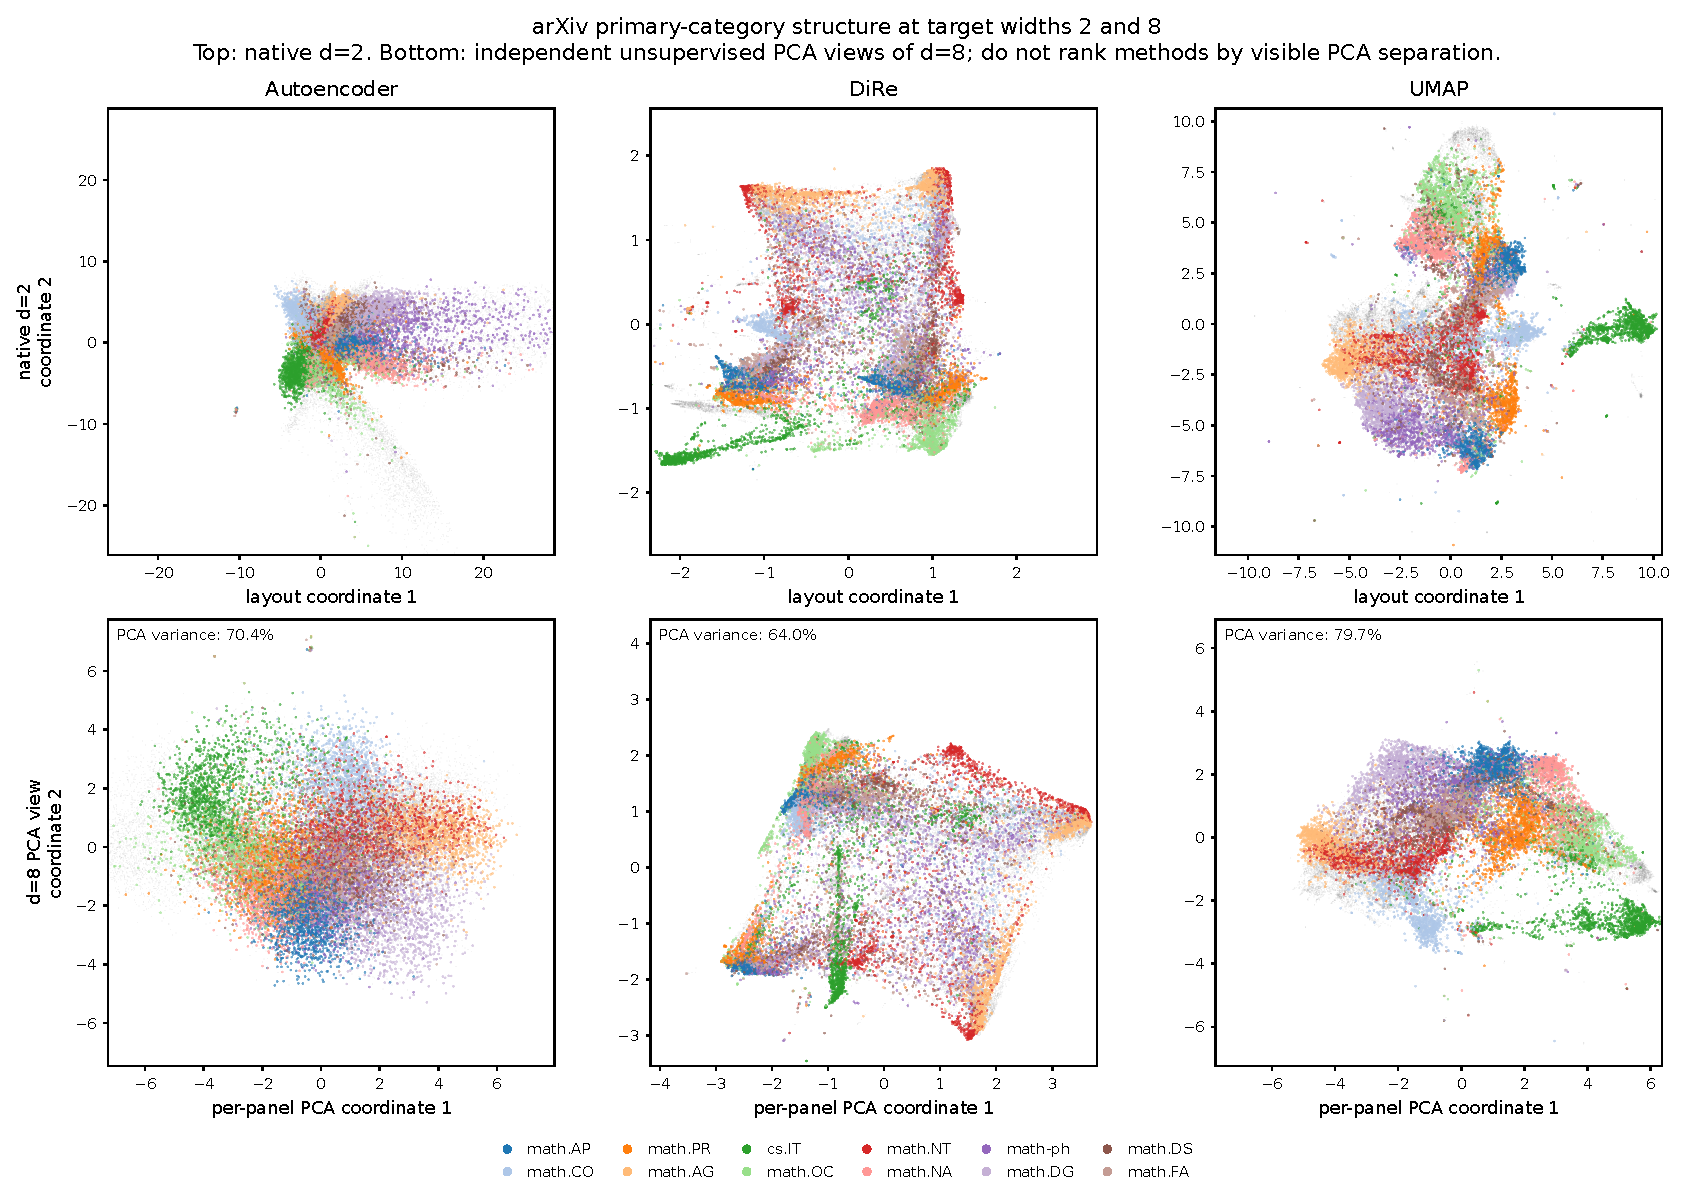
\includegraphics[width=\textwidth]{large_arxiv_category_layouts.pdf}
\caption{Seed-0 arXiv layouts at both target widths.  The top row is native $d=2$; the
bottom row is an independent unsupervised PCA view of each native $d=8$ layout, fitted on
the same uniform 100,000 rows.  Every panel uses 1,500 papers from each of the 12 largest
primary categories and a uniform 30,000-paper background outside those categories.
Colors and displayed indices are identical across widths and methods.  Coordinates and
isotropic robust limits are panel-specific; visible separation in the PCA row is not a
cross-method score.}
\label{fig:arxiv-layouts}
\end{figure}
\FloatBarrier

\subsection{Wikipedia: \texorpdfstring{$10^6\times1024\to\{2,8\}$}{1,000,000 x 1,024 to 2-D and 8-D}}

\begin{table}[H]
\centering
\scriptsize
\setlength{\tabcolsep}{3.0pt}
\resizebox{\textwidth}{!}{%
\begin{tabular}{rlrrrrrrrrrr}
\toprule
$d$ & Method & Fit (s)$\downarrow$ & Trust$\uparrow$ & Cont.$\uparrow$ & Overlap$\uparrow$
& $\rho_S\uparrow$ & Stress$\downarrow$ & Decode$\downarrow$
& Purity$\uparrow$ & Hit$\uparrow$ & TrRecall$\uparrow$\\
\midrule
2 & Autoencoder & 81.60 & \textbf{.887} & .827 & \textbf{.183}
& .230 & .747 & .907 & .006 & .050 & .006\\
2 & DiRe & \textbf{62.14} & .752 & .823 & .118
& .305 & \textbf{.428} & .959 & .136 & .288 & .141\\
2 & UMAP & 144.01 & .847 & \textbf{.832} & .182
& \textbf{.337} & .475 & \textbf{.907} & \textbf{.201} & \textbf{.498} & \textbf{.236}\\
\midrule
8 & Autoencoder & 81.85 & \textbf{.960} & \textbf{.944} & \textbf{.337}
& \textbf{.459} & .362 & \textbf{.791} & .071 & .283 & .079\\
8 & DiRe & \textbf{63.93} & .908 & .894 & .229
& .378 & \textbf{.268} & .844 & .306 & .570 & .345\\
8 & UMAP & 144.05 & .917 & .885 & .235
& .389 & .438 & .841 & \textbf{.410} & \textbf{.754} & \textbf{.530}\\
\bottomrule
\end{tabular}}
\caption{Wikipedia means over three reducer/training seeds at both target widths.
Boldface is assigned within each width.  Article purity, hit rate, and truncated recall
query 3,000 anchors against the complete one-million-row layout.  At width two, UMAP's
mean decoding NMSE is only $0.00003$ below the autoencoder's before rounding.}
\label{tab:wikipedia}
\end{table}

At width two, the autoencoder gives the highest trustworthiness and a narrowly higher
exact-neighbor overlap than UMAP; UMAP leads continuity, pair-distance ordering, the
shared decoding probe, and all three article-group scores; and DiRe gives the lowest
stress.  At width eight, the autoencoder wins every sample-conditional local-geometry
metric and the shared decoding probe.  It does not organize exact article groups as
strongly: UMAP
places at least one same-article paragraph among the first 16 neighbors for 75.4\% of
eligible anchors, compared with 57.0\% for DiRe and 28.3\% for the autoencoder.  DiRe
gives the lowest global stress at both widths.  Wikipedia thus has meaningful group labels, but they
express exact article identity rather than broad semantic categories.  The winning method
for every Table~\ref{tab:wikipedia} width-eight metric is unchanged across the three
seeds; the largest listed sample standard deviation is 0.018 for autoencoder stress.

All three reducers improve every reported Wikipedia quality metric when moving from two
to eight coordinates.  The autoencoder changes most sharply: stress falls from .747 to
.362, pair correlation doubles from .230 to .459, and article hit rate rises from .050
to .283.  UMAP remains the article-group leader at both widths, reaching .754 hit rate at
width eight.  The crossover therefore separates a target-width effect from the earlier
corpus comparison: the autoencoder's width-eight local-geometry advantage is not merely
a peculiarity of using Wikipedia rather than arXiv.

Figure~\ref{fig:wikipedia-layouts} shows the native width-two layouts and illustrative
PCA views of width eight.  The PCA panels' axes and visible separations cannot be treated
as the scored embedding.  Figure~\ref{fig:label-metrics} shows the native-layout retrieval
statistics over both widths and all three reducer seeds.

\begin{figure}[htbp]
\centering
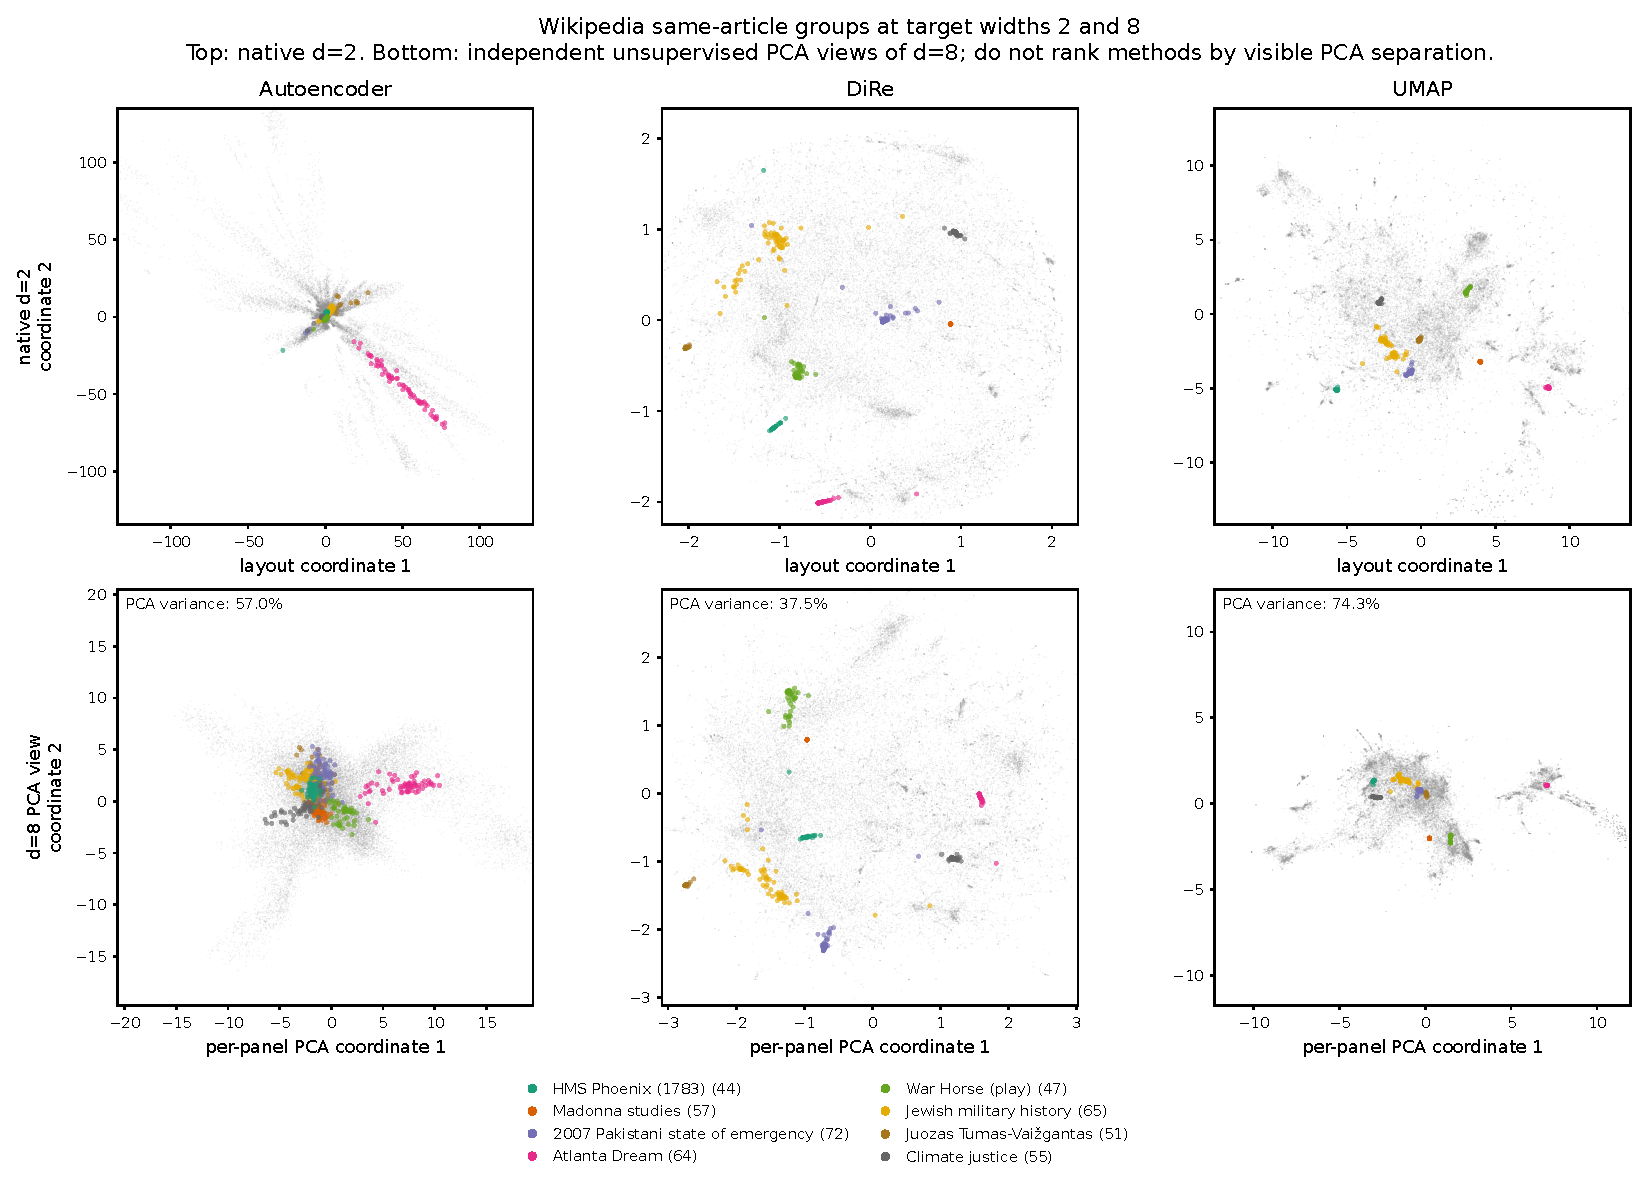
\includegraphics[width=\textwidth]{large_wikipedia_article_layouts.pdf}
\caption{Seed-0 Wikipedia layouts at both target widths.  The top row is native $d=2$;
the bottom row is an independent unsupervised PCA view of each native $d=8$ layout,
fitted on the same uniform 100,000 rows.  Eight articles containing 40--100 paragraphs
are chosen by a deterministic prespecified rule independent of all layouts, and every
paragraph from them is shown over the same 30,000-row background.  Highlighted and
background indices are identical across widths and methods.  Coordinates and isotropic
robust limits are panel-specific; displayed PCA variance is descriptive, and no
cross-method ranking should be inferred from the PCA row.}
\label{fig:wikipedia-layouts}
\end{figure}
\FloatBarrier

\begin{figure}[htbp]
\centering
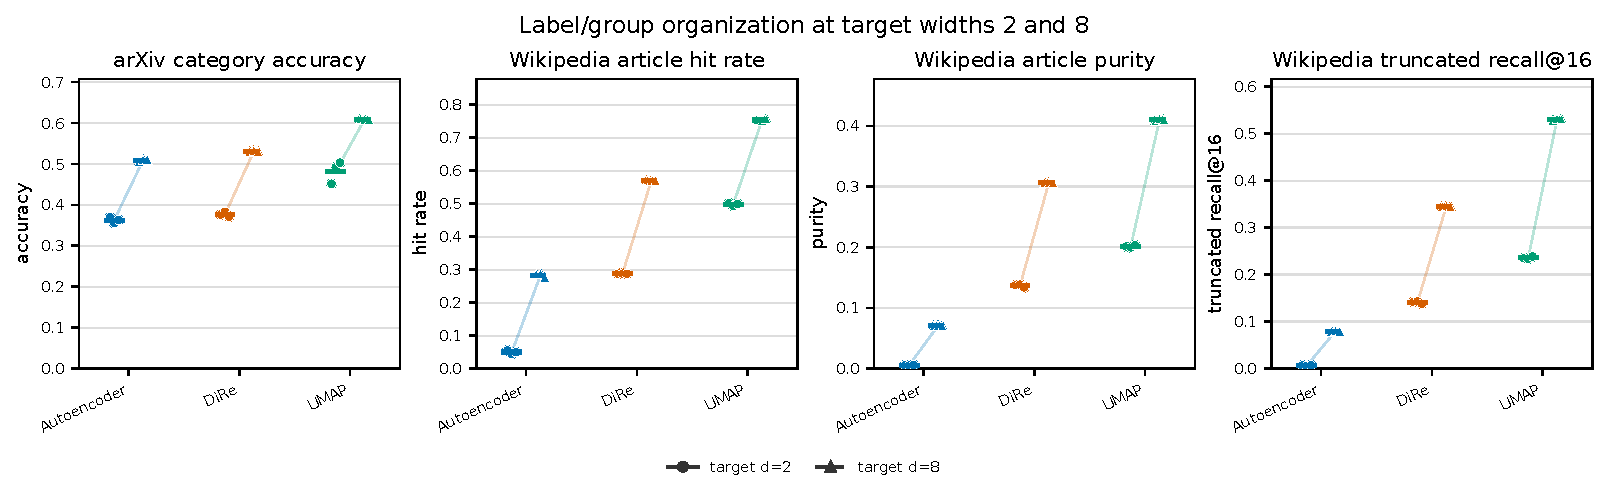
\includegraphics[width=\textwidth]{large_label_preservation_metrics.pdf}
\caption{Label/group organization in the native layouts.  Points are the three
reducer/training seeds and horizontal segments are means; circles and solid mean bars are
$d=2$, triangles and dashed bars are $d=8$, and faint segments join width means.  arXiv
uses category classification accuracy.  Wikipedia uses full-million-layout article hit
rate, purity, and truncated recall at 16 with the same 3,000 anchors at both widths.
These are native-layout metrics, not scores of the PCA views in
Figure~\ref{fig:wikipedia-layouts}.  Labels are evaluation-only and are not supplied to
any reducer.}
\label{fig:label-metrics}
\end{figure}
\FloatBarrier

\subsection{Sampled topology descriptions}

\begin{table}[ht]
\centering
\small
\begin{tabular}{lrlrr}
\toprule
Corpus & $d$ & Method & FastDTW($\beta_0$)$\downarrow$ & FastDTW($\beta_1$)$\downarrow$\\
\midrule
arXiv & 2 & Autoencoder & 4,841 & 439\\
      & 2 & DiRe & \textbf{3,322} & \textbf{176}\\
      & 2 & UMAP & 10,414 & 941\\
      & 8 & Autoencoder & \textbf{1,583} & 3,045\\
      & 8 & DiRe & 2,685 & \textbf{177}\\
      & 8 & UMAP & 6,469 & 499\\
\midrule
Wikipedia & 2 & Autoencoder & 4,822 & \textbf{8,974}\\
          & 2 & DiRe & \textbf{2,107} & 9,355\\
          & 2 & UMAP & 3,566 & 9,207\\
          & 8 & Autoencoder & \textbf{1,591} & \textbf{7,572}\\
          & 8 & DiRe & 3,335 & 9,117\\
          & 8 & UMAP & 2,986 & 9,198\\
\bottomrule
\end{tabular}
\caption{Pooled descriptive means across three reducer seeds and three evaluation samples.
Lower raw sequence discrepancy is preferable within a corpus and target width, subject
to the sampling, cloud-specific filtration grids, and FastDTW qualifications in the
text.}
\label{tab:topology}
\end{table}

At arXiv width two, DiRe has the lowest sampled $\beta_0$ and $\beta_1$ curve
discrepancies, and the autoencoder lies between DiRe and UMAP.  At width eight the result
splits: the autoencoder has the lowest $\beta_0$ discrepancy, while DiRe remains lowest
on $\beta_1$.  Increasing arXiv width lowers $\beta_0$ discrepancy for all three methods,
but $\beta_1$ is nearly unchanged for DiRe, improves for UMAP, and worsens substantially
for the autoencoder.  Wikipedia behaves differently.  At width two, DiRe has the lowest
$\beta_0$ discrepancy and the autoencoder the lowest $\beta_1$ discrepancy; at width
eight the autoencoder has the lowest value in both columns.  From width two to eight,
both autoencoder discrepancies fall, whereas DiRe's $\beta_0$ discrepancy rises and
UMAP's $\beta_1$ discrepancy is essentially unchanged.  Thus neither a wider target nor
one reducer has a corpus-independent topological advantage in these samples; the
rankings exhibit a corpus-by-width interaction.  Table~\ref{tab:topology} is a
descriptive sample comparison, not a claim that the reported values prove preservation
of the full-corpus homology.

\subsection{Local and reconstructive dimension estimates are related, not identical}

\begin{table}[ht]
\centering
\small
\begin{tabular}{lrrrr}
\toprule
Manifold & Known local $d$ & TwoNN & MLE ($k=20$) & AE elbow\\
\midrule
Rank-three linear & 3 & $3.036\pm0.094$ & $3.053\pm0.045$ & $3.000\pm0.000$\\
Circle & 1 & $1.034\pm0.061$ & $0.997\pm0.008$ & $2.000\pm0.000$\\
Swiss roll & 2 & $1.990\pm0.084$ & $1.929\pm0.033$ & $2.667\pm0.577$\\
\bottomrule
\end{tabular}
\caption{Controlled input-space intrinsic-dimension cross-check.  Entries are
mean$\pm$sample standard deviation across three independent data/model seeds.  The AE
elbows for the Swiss roll are 3, 3, and 2.  These synthetic results are not estimates for
the arXiv or Wikipedia corpora.}
\label{tab:id-crosscheck}
\end{table}

\begin{figure}[htbp]
\centering
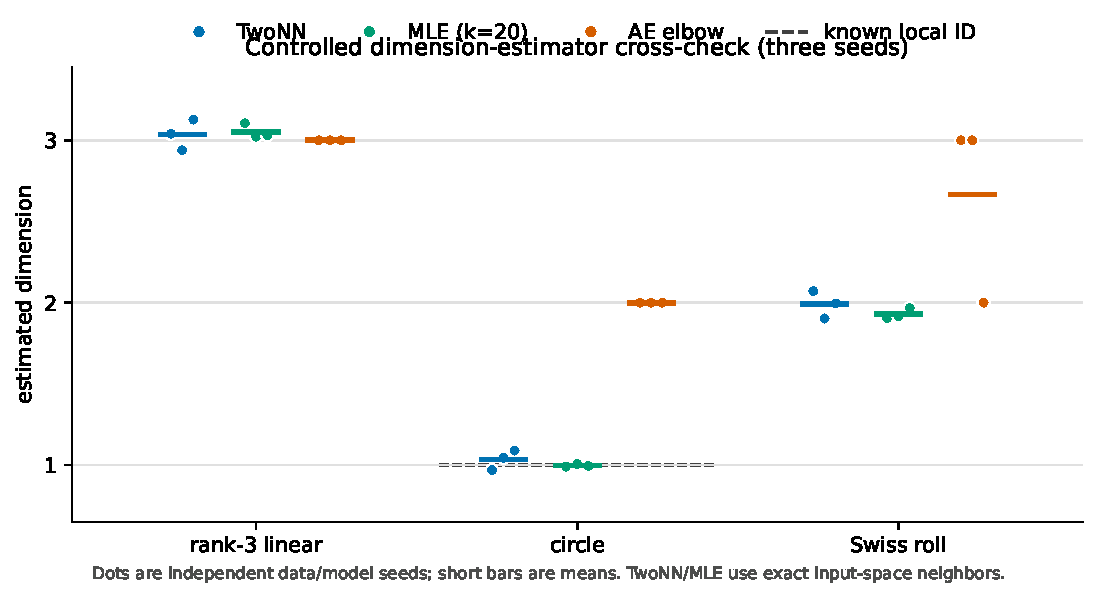
\includegraphics[width=0.82\textwidth]{dimension_estimator_agreement.pdf}
\caption{The three seeded estimates underlying Table~\ref{tab:id-crosscheck}.  Dots show
individual seeds, short horizontal segments show means, and dashed segments show known
local dimension.  TwoNN and MLE use exact input-space neighbors; the AE points are
accepted validation-reconstruction elbows.}
\label{fig:id-crosscheck}
\end{figure}
\FloatBarrier

Rounding TwoNN to the nearest integer, its estimate and the AE elbow agree exactly in
four of nine seeded trials and differ by at most one in all nine.  Their paired Spearman
correlation is $\rho_S=.779$.  This correlation is descriptive only: the nine pairs are
clustered within three deliberately chosen manifold families, so neither a null-model
$p$-value nor a population-level inference is warranted.

The pattern is more informative than the aggregate count.  Both estimators recover the
rank-three linear subspace.  The circle is locally one-dimensional, but a continuous
Euclidean autoencoder generally needs two coordinates to reconstruct it globally without
a cut, so its stable $1$ versus $2$ difference reflects the two estimands rather than a
failure.  A Swiss roll is locally two-dimensional and globally unrollable into a plane;
TwoNN recovers two, while finite-network optimization together with the chord-elbow rule
selects either two or three across seeds.  Thus the pointwise and neighbor-based approaches
do not produce unrelated notions of dimension, but topology, model capacity, optimization,
and elbow-rule sensitivity prevent an identity theorem.

\subsection{Why is the autoencoder so fast?}

\begin{table}[ht]
\centering
\small
\begin{tabular}{lrrrrrr}
\toprule
Corpus & $d$ & GPU staging & Epoch selection & Full refit & Encode/statistics & Total\\
\midrule
arXiv & 2 & 0.14 & 11.90 & 11.58 & 0.69 & 24.32\\
arXiv & 8 & 0.11 & 11.43 & 11.21 & 0.67 & 23.42\\
Wikipedia & 2 & 0.40 & 39.14 & 39.60 & 2.46 & 81.60\\
Wikipedia & 8 & 0.42 & 39.29 & 39.67 & 2.47 & 81.85\\
\bottomrule
\end{tabular}
\caption{Mean autoencoder fit-time decomposition in seconds.  The headline time includes
both training phases.}
\label{tab:timing}
\end{table}

The timing is less paradoxical than it first appears.  The arXiv and Wikipedia networks
are small, their complete 1.1 and 4.1 GB float32 matrices fit in GPU memory, and a batch
of 32,768 leaves only about 23 and 31 steps per epoch.  Approximately 400 epochs across
selection and refitting therefore require about 8,800 and 12,000 regular dense optimizer steps after
accounting for the 5\% selection holdout.  The primary results in
Table~\ref{tab:timing} use no mixed precision and include both the validation-selection
model and the fresh full-data model.

These are implementation measurements on a GH200, not hardware-independent complexity
constants.  The graph reducers also avoid quadratic behavior, but do so through
approximate indexing and sparse operations rather than dense GEMMs.

\subsection{BF16 sensitivity: tested margins pass, topology is mixed, and speed is
model-size dependent}

We repeated every autoencoder cell---both corpora, $d\in\{2,8\}$, and seeds 0--2---with
CUDA BF16 autocast during training, epoch-selection validation, and final encoding.
Parameters, gradients, AdamW state, the explicit MSE loss, and reconstruction
accumulations remained float32.  Inputs, samples, seeds, architecture, and optimizer
settings matched the primary runs.  These are paired sensitivity runs; the scientific
comparison tables remain the primary float32 results.

\begin{table}[ht]
\centering
\scriptsize
\setlength{\tabcolsep}{3.7pt}
\begin{tabular}{lrrrrrrrr}
\toprule
& & \multicolumn{3}{c}{Selection + refit training} &
\multicolumn{3}{c}{Complete reported fit} & Native NMSE\\
\cmidrule(lr){3-5}\cmidrule(lr){6-8}
Corpus & $d$ & FP32 (s) & BF16 (s) & Speedup & FP32 (s) & BF16 (s) & Speedup & BF16/FP32\\
\midrule
arXiv & 2 & 23.49 & 25.49 & 0.920$\times$ & 24.32 & 26.28 & 0.925$\times$ & 1.00193\\
arXiv & 8 & 22.64 & 25.46 & 0.889$\times$ & 23.42 & 26.25 & 0.892$\times$ & 1.00131\\
Wikipedia & 2 & 78.74 & 39.43 & 1.997$\times$ & 81.60 & 42.28 & 1.931$\times$ & 1.00096\\
Wikipedia & 8 & 78.96 & 41.53 & 1.901$\times$ & 81.85 & 44.34 & 1.846$\times$ & 1.00023\\
\bottomrule
\end{tabular}
\caption{Paired three-seed BF16 sensitivity.  Times are arithmetic means.  Speedup is
FP32 time divided by BF16 time; training speedup is the paired geometric mean and total
speedup is the paired arithmetic mean.  The displayed NMSE ratio is the arithmetic mean
of the three paired ratios.  Values below one indicate a BF16 slowdown.}
\label{tab:bf16}
\end{table}

Both the standard and FP32-evaluation-isolation BF16 arms pass all prespecified practical
checks on native reconstruction and shared geometry or label metrics in every cell; with
only three seeds these margins are descriptive, not formal equivalence tests.  The
largest paired BF16/FP32 native-NMSE ratio in the standard arm is 1.00243.
The sampled-topology response is mixed rather than uniformly invariant.  Pooled
$(\beta_0,\beta_1)$ DTW means change from $(4841,439)$ to $(5660,537)$ for arXiv
$d=2$, from $(1583,3045)$ to $(1659,3068)$ for arXiv $d=8$, from $(4822,8974)$ to
$(4820,8986)$ for Wikipedia $d=2$, and from $(1591,7572)$ to $(1505,8121)$ for
Wikipedia $d=8$.  A clean rerun that trained with BF16 but performed validation,
encoding, reconstruction, shared-metric evaluation, and topology input generation in
float32 left shared-metric quality essentially unchanged and moved the pooled topology
mean closer to FP32 in only four of eight corpus--width--Betti comparisons.  Thus
this descriptive isolation does not support final-coordinate quantization as the main
explanation for the topology differences.

A 100-step resident-batch microprofile explains why a universal three- or four-fold
speedup does not appear.  With TF32 matrix multiplication disabled, this fixed-order
profile uses a synthetic standard-normal resident batch and separate warm-ups for each
precision.  Its FP32/BF16 total-step speedups are 0.859 and 0.842 for the two arXiv
widths, versus 2.407 and 2.428 for Wikipedia; the Wikipedia forward-plus-backward portion
alone reaches about $2.65\times$.  The approximately 272,000-parameter arXiv MLP is
overhead-bound at this batch shape, so autocast dispatch and conversions outweigh faster
eligible kernels.  The roughly 1.35-million-parameter Wikipedia MLP supplies enough
dense matrix work to benefit, although FP32 AdamW and the non-training parts of the fit
cap the end-to-end gain near $1.85$--$1.93\times$.  Because the full-fit FP32 runs and
later BF16 runs were not alternated contemporaneously, their timing ratios are
descriptive; the microprofile independently reproduces the workload crossover.

\subsection{Longer MSE optimization is not a geometry rule}

\begin{table}[ht]
\centering
\scriptsize
\setlength{\tabcolsep}{3.2pt}
\resizebox{\textwidth}{!}{%
\begin{tabular}{llrrrrrrrr}
\toprule
Corpus & Run & Native NMSE$\downarrow$ & Trust$\uparrow$ & Cont.$\uparrow$
& Overlap$\uparrow$ & $\rho_S\uparrow$ & Stress$\downarrow$
& DTW $\beta_0\downarrow$ & DTW $\beta_1\downarrow$\\
\midrule
arXiv & primary (199 epochs) & .5965 & .8818 & .9140 & .1006 & .5925 & .5615 & 4,544 & 516\\
arXiv & longer (398 epochs) & .5753 & .8940 & .9091 & .1135 & .5746 & .6955 & 5,771 & 772\\
Wikipedia & primary (200 epochs) & .6910 & .9600 & .9426 & .3339 & .4593 & .3818 & 1,599 & 8,146\\
Wikipedia & longer (400 epochs) & .6744 & .9629 & .9396 & .3460 & .4517 & .3969 & 1,545 & 9,709\\
\bottomrule
\end{tabular}}
\caption{Reducer-seed-0 400-epoch-cap sensitivity checks for the two original benchmark
cells only: arXiv $d=2$ and Wikipedia $d=8$.  DTW columns average the three fixed
evaluation samples.  Longer training lowers native reconstruction error and improves
some local scores, while several global and sampled-topology scores worsen.}
\label{tab:sensitivity}
\end{table}

For these two original cells, reconstruction convergence is therefore not a universal
stopping criterion for a useful layout.  Longer training improves native MSE,
trustworthiness, and exact overlap, but reduces continuity and pair-rank correlation,
worsens stress, and gives mixed or worse sampled Betti-curve discrepancies.  No analogous
400-epoch claim is made for the crossed target widths.  A geometry-aware autoencoder
objective might change this tradeoff, but it would also move away from the deliberately
simple pointwise MSE experiment studied here.

\section{Conclusions and limitations}

The reducer results support six narrow conclusions.
\begin{enumerate}
  \item A small MSE autoencoder is computationally practical at 723,000--1,000,000 rows
        in this GH200 configuration.  Its favorable timing is consistent with
        fixed-architecture linear-in-$N$ pointwise work and efficient dense kernels.
        BF16 autocast passes the tested reconstruction and shared-metric practical
        margins, while its sampled-topology response is mixed.  Its speed is
        shape-dependent: it nearly halves Wikipedia training time and slightly slows the
        smaller arXiv model.
  \item Plain reconstruction can preserve sampled local geometry and decodability very
        well without an explicit pairwise objective.  This does not guarantee strong
        label/group organization: UMAP wins arXiv category prediction at both widths and
        Wikipedia same-article retrieval at both widths.
  \item On both corpora, increasing $d$ from two to eight changes local-fidelity rankings
        as well as score magnitudes: the autoencoder leads the local, distance-order, and
        decoding columns at width eight but not at width two.  DiRe retains the best
        Wikipedia stress.  This repeated contrast supports a target-width effect within
        the tested settings, not a general scaling law.
  \item Controlled known-manifold checks show approximate rather than exact agreement
        between TwoNN local dimension and the AE reconstruction elbow.  Their systematic
        circle difference illustrates why local and global reconstructive dimension must
        be interpreted separately.
  \item More MSE optimization is not automatically better dimension reduction.
        Reconstruction, local ranks, global distances, labels, and sampled topology can
        move in different directions in the two original sensitivity cells.
  \item Sampled topology has no universal method or width ordering here.  The arXiv
        width-eight autoencoder improves markedly in $\beta_0$ but worsens in $\beta_1$;
        the Wikipedia width-eight autoencoder improves in both.  These completed cells
        point to a corpus-by-width interaction rather than a single topological winner.
\end{enumerate}

The comparison has important limits.  It uses one accelerator, one architecture family,
one neighborhood size, and only two target widths.  arXiv category labels and Wikipedia
URL groups have different meanings.  All primary layouts are transductive, and the
autoencoder is retrained for every corpus, width, and seed.  Neighborhood metrics are
sample-conditional; distance metrics use sampled pairs; topology uses small sampled
clouds and cloud-specific curve grids.  The three-seed comparisons are descriptive, not
formal uncertainty quantification, and two target widths cannot identify a general
dimension-response curve.  The controlled dimension check uses small synthetic
manifolds and does not estimate the intrinsic dimension of either text corpus.

\section*{Reproducibility}

The companion \emph{dimension-reduction-benchmarks} repository
\cite{benchmarkrepo} provides the benchmark,
topology, and controlled-dimension implementations together with compact result tables
and machine-readable figure provenance.  The supplementary records retain exact
environment information, checksums, sample identities, and complete topology curves;
those audit identifiers are intentionally kept out of the public-facing narrative.

\begin{thebibliography}{12}
\bibitem{hinton2006}
G.~E. Hinton and R.~R. Salakhutdinov,
``Reducing the dimensionality of data with neural networks,''
\emph{Science} 313 (2006), 504--507.

\bibitem{umap}
L. McInnes, J. Healy, and J. Melville,
``UMAP: Uniform Manifold Approximation and Projection for Dimension Reduction,''
arXiv:1802.03426 (2018).

\bibitem{dire}
A. Kolpakov and I. Rivin,
``Dimensionality reduction for homological stability and global structure preservation,''
arXiv:2503.03156 (2025),
\url{https://doi.org/10.48550/arXiv.2503.03156}.

\bibitem{facco2017}
E. Facco, M. d'Errico, A. Rodriguez, and A. Laio,
``Estimating the intrinsic dimension of datasets by a minimal neighborhood information,''
\emph{Scientific Reports} 7 (2017), 12140.

\bibitem{levina2004}
E. Levina and P. J. Bickel,
``Maximum likelihood estimation of intrinsic dimension,''
in \emph{Advances in Neural Information Processing Systems 17} (2004), pp. 777--784.

\bibitem{trust}
J. Venna and S. Kaski,
``Neighborhood preservation in nonlinear projection methods: an experimental study,''
in \emph{Artificial Neural Networks---ICANN 2001}, pp. 485--491.

\bibitem{ripser}
U. Bauer,
``Ripser: efficient computation of Vietoris--Rips persistence barcodes,''
\emph{Journal of Applied and Computational Topology} 5 (2021), 391--423.

\bibitem{fastdtw}
S. Salvador and P. Chan,
\emph{Toward accurate dynamic time warping in linear time and space},
\emph{Intelligent Data Analysis} 11 (2007), 561--580.

\bibitem{bge}
Beijing Academy of Artificial Intelligence,
\emph{BGE small English v1.5},
\url{https://huggingface.co/BAAI/bge-small-en-v1.5} (2023).

\bibitem{coherewiki}
Cohere Labs,
\emph{Wikipedia 2023-11 multilingual-v3 embeddings},
\href{https://huggingface.co/datasets/CohereLabs/wikipedia-2023-11-embed-multilingual-v3}
{Hugging Face dataset card} (accessed July 2026).

\bibitem{benchmarkrepo}
I. Rivin,
\emph{dimension-reduction-benchmarks: autoencoder, DiRe, and UMAP experiments},
\url{https://github.com/igorrivin/dimension-reduction-benchmarks} (2026).
\end{thebibliography}

\end{document}
